\setcounter{topnumber}{5}
\setcounter{bottomnumber}{5}
\setcounter{totalnumber}{5}

\chapter{Desenvolvimento}
\section{Fundamentação Teórica}
\begin{enumerate}
	\item Diagrama de bode
	\item Resposta em frequência
	\item Explicar um filtro passa baixa, passa alta, rejeita faixa e passa faixa (um exemplo prático desta aplicação) \ldots
\end{enumerate}



\newpage
\section{Procedimentos}


\subsection{Amplificador $ 1^\circ $ estágio}

\centerline{\begin{minipage}[c]{\textwidth}
		\centering
		\noindent
		\captionof{figure}{Circuito elétrico do $ 1^\circ $ estágio do amplificador}
		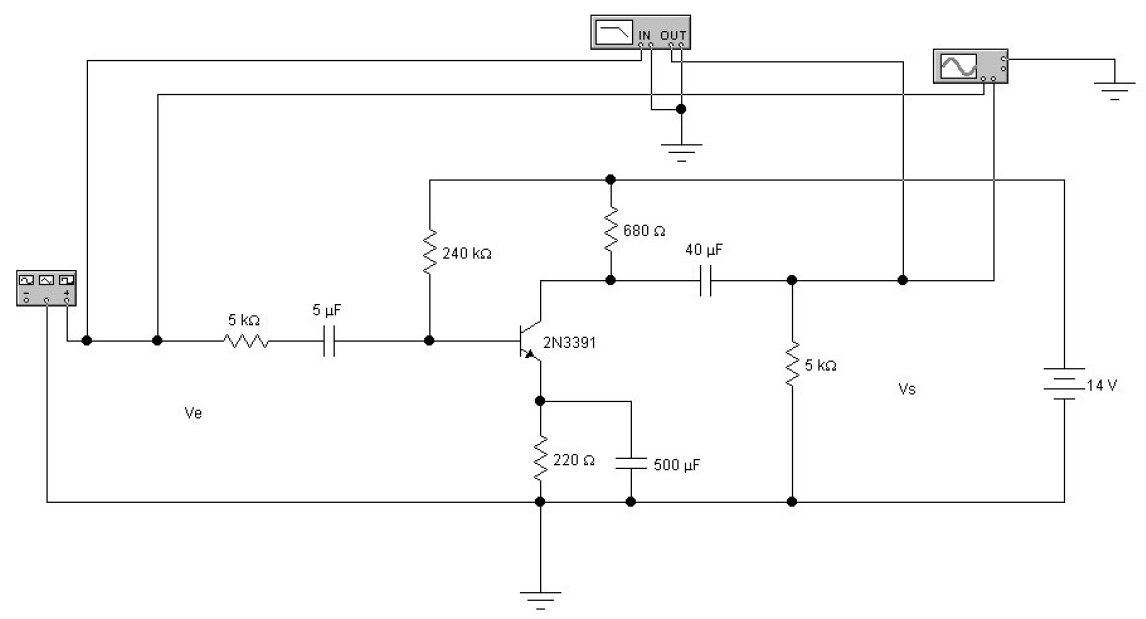
\includegraphics[width=0.9\textwidth]{Imagens/Figura1.jpg}
		\legend{Fonte: Produzido pelos autores}
		\label{Figura1}
\end{minipage}}
	
\begin{enumerate}
	\item Dado o circuito da figura \ref{Figura1}, aplicar o gerador de funções com uma tensão $ 1,0mV $ e frequência de $ 1kHz $;
	\item Medir o ganho com o osciloscópio. Para tanto medir a tensão de saída $ V_s $ e de entrada $ V_e $.
	\item Usar o Bode Plotter (amplitude) e medir as frequências de corte e o ganho da banda passante em $ dB $ $ A $ $ db = 20 \log (V_s/V_e) $;
	\item Usar o Bode Plotter (fase) e medir os ângulos nas frequências importantes; Anotar todos os dados obtidos na tabela \ref{Tabela1}.
\end{enumerate}


\subsection{Amplificador $ 2^\circ $ estágio}

\centerline{\begin{minipage}[c]{\textwidth}
		\centering
		\noindent
		\captionof{figure}{Circuito elétrico do $ 2^\circ $ estágio do amplificador}
		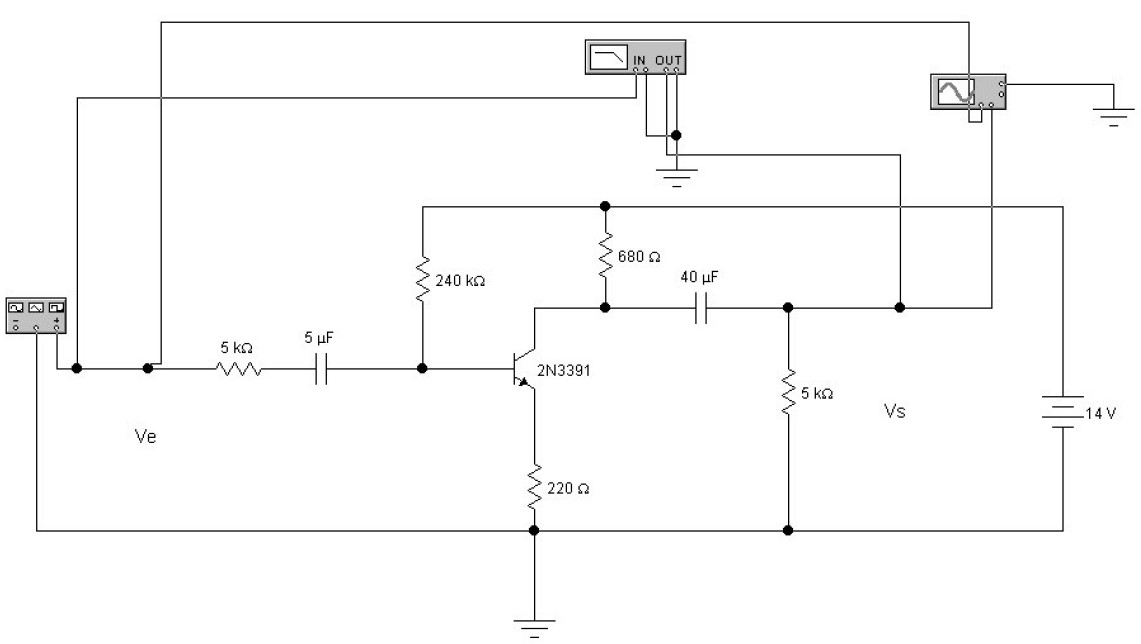
\includegraphics[width=0.9\textwidth]{Imagens/Figura2.jpg}
		\legend{Fonte: Produzido pelos autores}
		\label{Figura2}
\end{minipage}}

\begin{enumerate}
	\item Dado o circuito figura \ref{Figura2}, aplicar o gerador de funções com uma tensão $ 1,0mV $ e frequência de $ 1kHz $;
	\item Medir o ganho com o osciloscópio. Para tanto medir a tensão de saída $ V_s $ e de entrada $ V_e $.
	\item Usar o Bode Plotter (amplitude) e medir as frequências de corte e o ganho da banda passante em $ dB $;
	\item Usar o Bode Plotter (fase) e medir os ângulos nas frequências importantes; Anotar todos os dados obtidos na tabela \ref{Tabela1}.
\end{enumerate}

\subsection{Amplificador com dois estágios}

\centerline{\begin{minipage}[c]{\textwidth}
		\centering
		\noindent
		\captionof{figure}{Circuito elétrico do amplificador com dois estágios}
		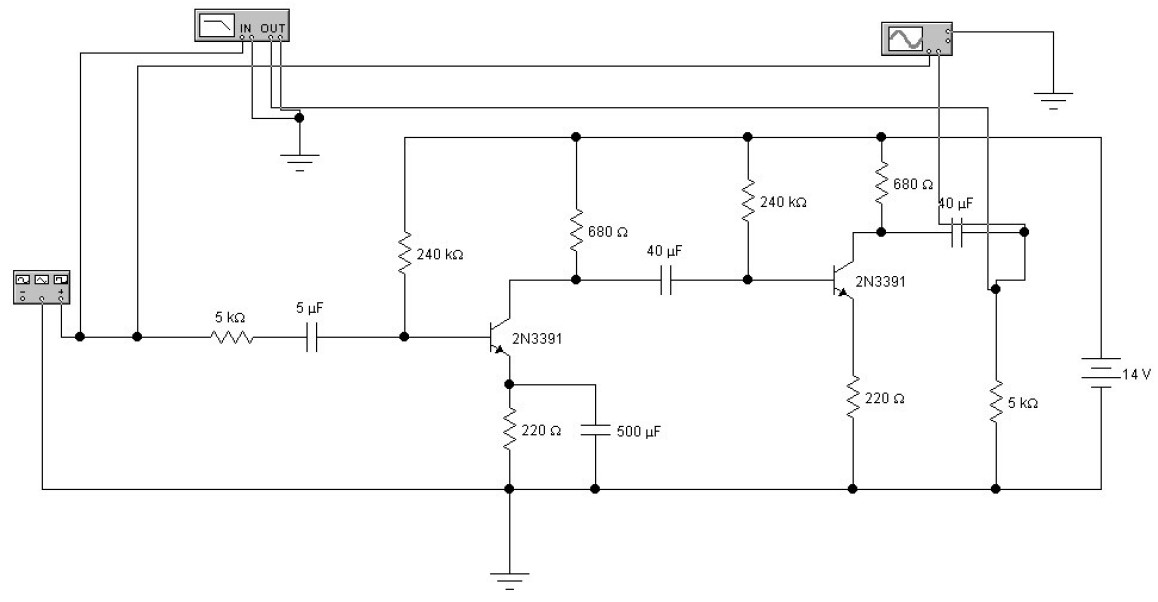
\includegraphics[width=0.9\textwidth]{Imagens/Figura3.jpg}
		\legend{Fonte: Produzido pelos autores}
		\label{Figura3}
\end{minipage}}

\begin{enumerate}
	\item Dado o circuito figura \ref{Figura3}, aplicar o gerador de funções com uma tensão $ 1,0mV $ e frequência de $ 1kHz $;
	\item Medir o ganho com o osciloscópio. Para tanto medir a tensão de saída $ V_s $ e de entrada $ V_e $.
	\item Usar o Bode Plotter (amplitude) e medir as frequências de corte e o ganho da banda passante em $ dB $;
\end{enumerate}

\subsection{Analise}
\begin{enumerate}
	\item Analise os resultados apontados na Tabela \ref{Tabela2} e explique:
	\begin{enumerate}
		\item Por que a frequência de corte inferior $ (fr_1) $ para o circuito da figura \ref{Figura1} é maior que para o circuito da figura \ref{Figura2}?
		\item Por que o ganho, para a faixa de frequência médias, do circuito da figura \ref{Figura1} é bem maior do que o circuito da figura \ref{Figura2}?
	\end{enumerate}
\end{enumerate}

\centerline{\begin{minipage}[c]{\textwidth}
		\centering
		\noindent
		\captionof{table}{Valores obtidos dos circuitos}
		\begin{tabular}{ll|c|c|l|}
			\cline{3-5}
			&     & Circuito $ 1 $ & Circuito $ 2 $ & Circuito $ 3 $ \\ \hline
			\multicolumn{1}{|c|}{\multirow{3}{*}{Osciloscópio}} & $V_e$ $ (V_{pp}) $   &            &            &            \\ \cline{2-5} 
			\multicolumn{1}{|c|}{}                              & $V_s$ $ (V_{pp}) $   &            &            &            \\ \cline{2-5} 
			\multicolumn{1}{|c|}{}                              & $A_V$ $ (V_s/V_e) $   &            &            &            \\ \hline
			\multicolumn{1}{|l|}{\multirow{3}{*}{Bode Plotter}} & $A_V$ em frequências médias $ (dB) $   &            &            &            \\ \cline{2-5} 
			\multicolumn{1}{|l|}{}                              & frequência $ 1 $ a $ (-3dB) $ &            &            &            \\ \cline{2-5} 
			\multicolumn{1}{|l|}{}                              & frequência $ 2 $ a $ (-3dB) $ &            &            &            \\ \hline
		\end{tabular}
		\legend{Fonte: Produzido pelos autores}
		\label{Tabela1}
\end{minipage}}

\newpage
\section{Resultados}

\subsection{Amplificador $ 1^\circ $ estágio}
Temos a seguinte montagem do circuito da figura \ref{Figura1} com a utilização do MULTISIM:


\begin{center}
	\textbf{--- ADD a imagem - Simulação\_Circuito1.png ---}
\end{center}

Com a utilização do Osciloscópio do simulador, conseguimos obter a forma de onda da entrada e da saída, que para uma melhor visualização deixando as duas formas de onda com escalas diferentes.

\centerline{\begin{minipage}[c]{\textwidth}
		\centering
		\noindent
		\captionof{figure}{Imagem do osciloscópio do Circuito \ref{Figura1}}
		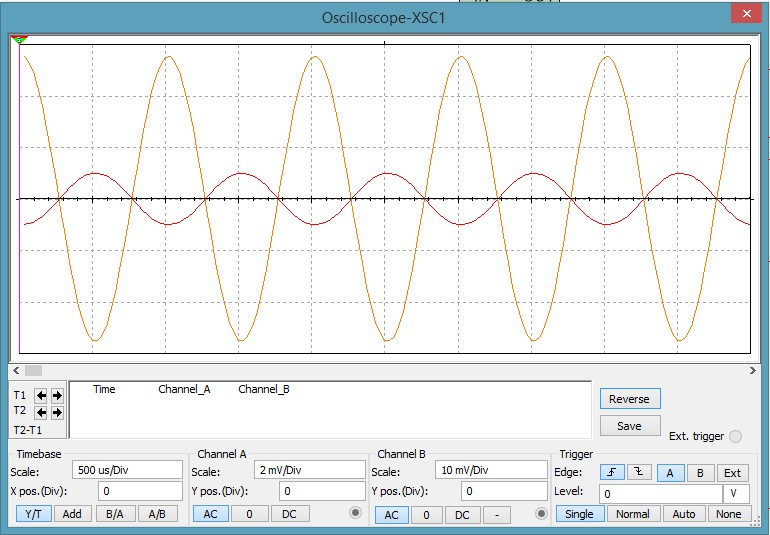
\includegraphics[width=0.9\textwidth]{Imagens/Oscilloscope_Circuito1.jpg}
		\legend{Fonte: Produzido pelos autores}
		\label{Oscilloscope_Circuito1}
\end{minipage}}

Usando o Bode Plotter, conseguimos analisar o gráfico do ganho em relação a frequência do circuito.

\centerline{\begin{minipage}[c]{\textwidth}
		\centering
		\noindent
		\captionof{figure}{Bode Plotter do Circuito \ref{Figura1}}
		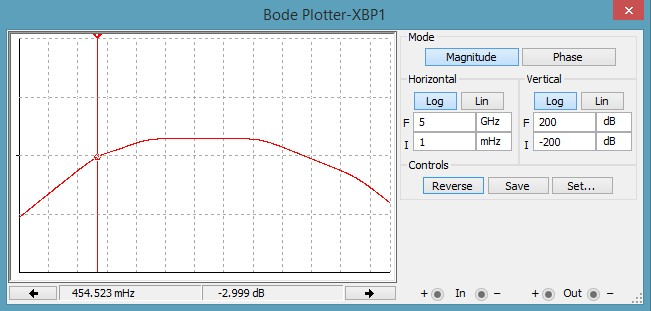
\includegraphics[width=0.9\textwidth]{Imagens/BodePlotter_Circuito1_Parte1.jpg}
		\legend{Fonte: Produzido pelos autores}
		\label{BodePlotter_Circuito1_Parte1}
\end{minipage}}

\centerline{\begin{minipage}[c]{\textwidth}
		\centering
		\noindent
		\captionof{figure}{Bode Plotter do Circuito \ref{Figura1}}
		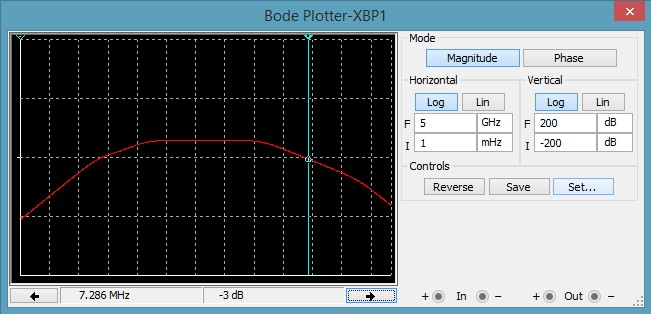
\includegraphics[width=0.9\textwidth]{Imagens/BodePlotter_Circuito1_Parte2.jpg}
		\legend{Fonte: Produzido pelos autores}
		\label{BodePlotter_Circuito1_Parte2}
\end{minipage}}

Com as informações encontradas, obtemos a seguintes informações:

\centerline{\begin{minipage}[c]{\textwidth}
		\centering
		\noindent
		\captionof{table}{Valores obtidos do circuito \ref{Figura1}}
	\begin{tabular}{ll|c|}
		\cline{3-3}
		&     & Circuito 1 \\ \hline
		\multicolumn{1}{|c|}{\multirow{3}{*}{Osciloscópio}} &  $V_e$ $ (V_{pp}) $    &   $ 2mV $         \\ \cline{2-3} 
		\multicolumn{1}{|c|}{}                              & $V_s$ $ (V_{pp}) $   &       $ 55,1mV $     \\ \cline{2-3} 
		\multicolumn{1}{|c|}{}                              &  $A_V$ $ (V_s/V_e) $   &      $ 27,55 $      \\ \hline
		\multicolumn{1}{|l|}{\multirow{3}{*}{Bode Plotter}} & $A_V$ em frequências médias $ (dB) $   &       $ 28,8 dB $     \\ \cline{2-3} 
		\multicolumn{1}{|l|}{}                              & frequência $ 1 $ a $ (-3dB) $ &      $ 454,523mHz  $  \\ \cline{2-3} 
		\multicolumn{1}{|l|}{}                              & frequência $ 2 $ a $ (-3dB) $ &        $ 7,286MHz $    \\ \hline
	\end{tabular}
		\legend{Fonte: Produzido pelos autores}
		\label{Tab_Circuito1}
\end{minipage}}

\subsection{Amplificador $ 2^\circ $ estágio}
Temos a seguinte montagem do circuito da figura \ref{Figura2} com a utilização do MULTISIM:


\begin{center}
	\textbf{--- ADD a imagem - Simulação\_Circuito2.png ---}
\end{center}

Com a utilização do Osciloscópio do simulador, conseguimos obter a forma de onda da entrada e da saída, que para uma melhor visualização deixando as duas formas de onda com escalas diferentes.


\centerline{\begin{minipage}[c]{\textwidth}
		\centering
		\noindent
		\captionof{figure}{Imagem do osciloscópio do Circuito \ref{Figura2}}
		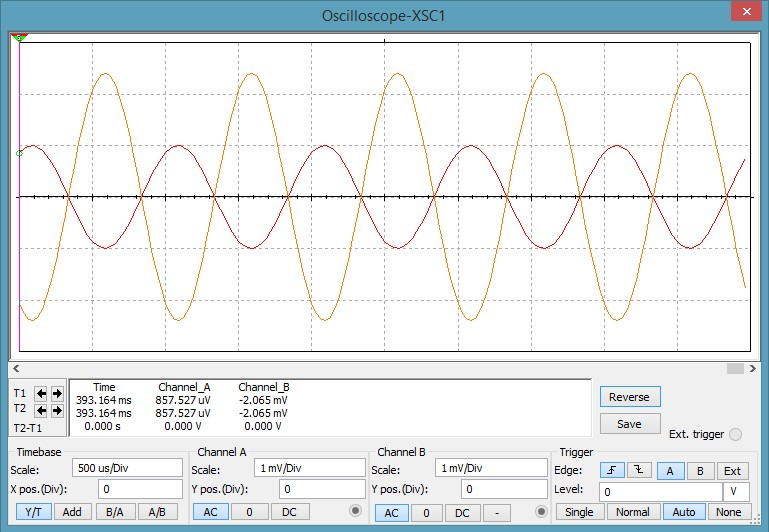
\includegraphics[width=0.9\textwidth]{Imagens/Oscilloscope_Circuito2.jpg}
		\legend{Fonte: Produzido pelos autores}
		\label{Oscilloscope_Circuito2}
\end{minipage}}

Usando o Bode Plotter, conseguimos analisar o gráfico do ganho em relação a frequência do circuito.

\centerline{\begin{minipage}[c]{\textwidth}
		\centering
		\noindent
		\captionof{figure}{Bode Plotter do Circuito \ref{Figura2}}
		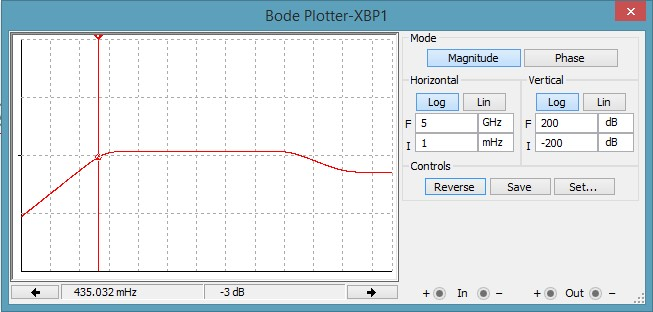
\includegraphics[width=0.9\textwidth]{Imagens/BodePlotter_Circuito2_Parte1.jpg}
		\legend{Fonte: Produzido pelos autores}
		\label{BodePlotter_Circuito2_Parte1}
\end{minipage}}

\centerline{\begin{minipage}[c]{\textwidth}
		\centering
		\noindent
		\captionof{figure}{Bode Plotter do Circuito \ref{Figura2}}
		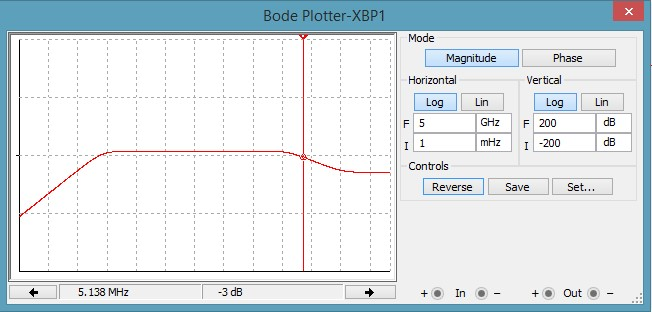
\includegraphics[width=0.9\textwidth]{Imagens/BodePlotter_Circuito2_Parte2.jpg}
		\legend{Fonte: Produzido pelos autores}
		\label{BodePlotter_Circuito2_Parte2}
\end{minipage}}

Com as informações encontradas, obtemos a seguintes informações:

\centerline{\begin{minipage}[c]{\textwidth}
		\centering
		\noindent
		\captionof{table}{Valores obtidos do circuito \ref{Figura2}}
		\begin{tabular}{ll|c|}
			\cline{3-3}
			&     & Circuito 2 \\ \hline
			\multicolumn{1}{|c|}{\multirow{3}{*}{Osciloscópio}} &  $V_e$ $ (V_{pp}) $    &   $ 2mV $         \\ \cline{2-3} 
			\multicolumn{1}{|c|}{}                              & $V_s$ $ (V_{pp}) $   &       $ 4,81mV $     \\ \cline{2-3} 
			\multicolumn{1}{|c|}{}                              &  $A_V$ $ (V_s/V_e) $   &      $ 2,405 $      \\ \hline
			\multicolumn{1}{|l|}{\multirow{3}{*}{Bode Plotter}} & $A_V$ em frequências médias $ (dB) $   &       $ 7,62 dB $     \\ \cline{2-3} 
			\multicolumn{1}{|l|}{}                              & frequência $ 1 $ a $ (-3dB) $ &      $ 435,032mHz  $  \\ \cline{2-3} 
			\multicolumn{1}{|l|}{}                              & frequência $ 2 $ a $ (-3dB) $ &        $ 5,138MHz $    \\ \hline
		\end{tabular}
		\legend{Fonte: Produzido pelos autores}
		\label{Tab_Circuito2}
\end{minipage}}

\subsection{Amplificador com dois estágios}

Temos a seguinte montagem do circuito da figura \ref{Figura3} com a utilização do MULTISIM:


\begin{center}
	\textbf{--- ADD a imagem - Simulação\_Circuito3.png ---}
\end{center}

Com a utilização do Osciloscópio do simulador, conseguimos obter a forma de onda da entrada e da saída, que para uma melhor visualização deixando as duas formas de onda com escalas diferentes.

\centerline{\begin{minipage}[c]{\textwidth}
		\centering
		\noindent
		\captionof{figure}{Imagem do osciloscópio do Circuito \ref{Figura3}}
		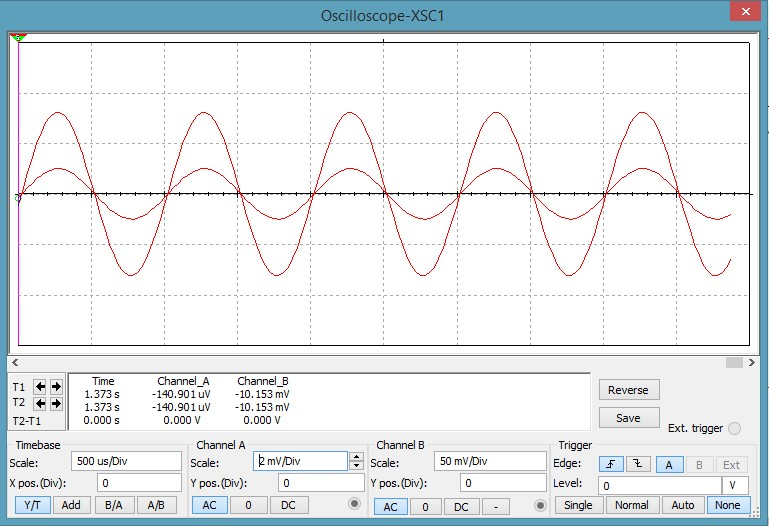
\includegraphics[width=0.9\textwidth]{Imagens/Oscilloscope_Circuito3.jpg}
		\legend{Fonte: Produzido pelos autores}
		\label{Oscilloscope_Circuito3}
\end{minipage}}

Usando o Bode Plotter, conseguimos analisar o gráfico do ganho em relação a frequência do circuito.

\centerline{\begin{minipage}[c]{\textwidth}
		\centering
		\noindent
		\captionof{figure}{Bode Plotter do Circuito \ref{Figura3}}
		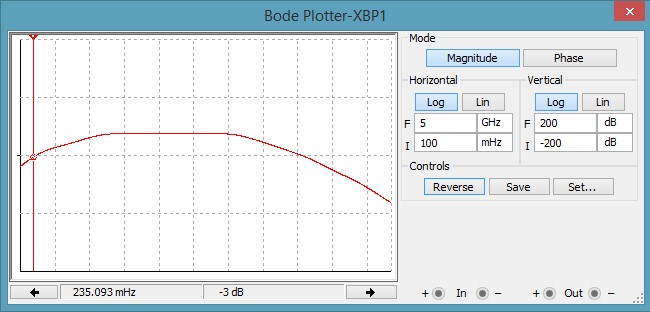
\includegraphics[width=0.9\textwidth]{Imagens/BodePlotter_Circuito3_Parte1.jpg}
		\legend{Fonte: Produzido pelos autores}
		\label{BodePlotter_Circuito3_Parte1}
\end{minipage}}

\centerline{\begin{minipage}[c]{\textwidth}
		\centering
		\noindent
		\captionof{figure}{Bode Plotter do Circuito \ref{Figura3}}
		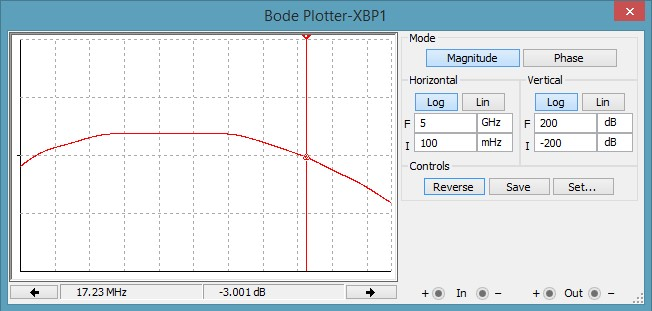
\includegraphics[width=0.9\textwidth]{Imagens/BodePlotter_Circuito3_Parte2.jpg}
		\legend{Fonte: Produzido pelos autores}
		\label{BodePlotter_Circuito3_Parte2}
\end{minipage}}

Com as informações encontradas, obtemos a seguintes informações:

\centerline{\begin{minipage}[c]{\textwidth}
		\centering
		\noindent
		\captionof{table}{Valores obtidos do circuito \ref{Figura3}}
		\begin{tabular}{ll|c|}
			\cline{3-3}
			&     & Circuito 3 \\ \hline
			\multicolumn{1}{|c|}{\multirow{3}{*}{Osciloscópio}} &  $V_e$ $ (V_{pp}) $    &   $ 2mV $         \\ \cline{2-3} 
			\multicolumn{1}{|c|}{}                              & $V_s$ $ (V_{pp}) $   &       $ 162mV $     \\ \cline{2-3} 
			\multicolumn{1}{|c|}{}                              &  $A_V$ $ (V_s/V_e) $   &      $ 81 $      \\ \hline
			\multicolumn{1}{|l|}{\multirow{3}{*}{Bode Plotter}} & $A_V$ em frequências médias $ (dB) $   &       $ 38,17 dB $     \\ \cline{2-3} 
			\multicolumn{1}{|l|}{}                              & frequência $ 1 $ a $ (-3dB) $ &      $ 235,093mHz  $  \\ \cline{2-3} 
			\multicolumn{1}{|l|}{}                              & frequência $ 2 $ a $ (-3dB) $ &        $ 17,23MHz $    \\ \hline
		\end{tabular}
		\legend{Fonte: Produzido pelos autores}
		\label{Tab_Circuito3}
\end{minipage}}

\subsection{Análise}
Para facilitar a análise, juntamos as informações obtidas de cada circuito numa tabela só.

\centerline{\begin{minipage}[c]{\textwidth}
		\centering
		\noindent
		\captionof{table}{Valores obtidos dos circuitos}
		\begin{tabular}{ll|c|c|c|}
			\cline{3-5}
			&     & Circuito $ 1 $ & Circuito $ 2 $ & Circuito $ 3 $ \\ \hline
			\multicolumn{1}{|c|}{\multirow{3}{*}{Osciloscópio}} & $V_e$ $ (V_{pp}) $   &$ 2mV $&$ 2mV $&$ 2mV $\\ \cline{2-5} 
			\multicolumn{1}{|c|}{}                              & $V_s$ $ (V_{pp}) $   &$ 55,1mV $&$ 4,81mV $&$ 162mV $            \\ \cline{2-5} 
			\multicolumn{1}{|c|}{}                              & $A_V$ $ (V_s/V_e) $   &$ 27,55 $&$ 2,405 $&   $ 81 $         \\ \hline
			\multicolumn{1}{|l|}{\multirow{3}{*}{Bode Plotter}} & $A_V$ em frequências médias $ (dB) $   &$ 28,8dB $&$ 7,62dB $ &$ 38,17 dB $ \\ \cline{2-5} 
			\multicolumn{1}{|l|}{}                              & frequência $ 1 $ a $ (-3dB) $ &$ 454,523mHz $&$ 435,032mHz $& $ 235,093mHz  $  \\ \cline{2-5} 
			\multicolumn{1}{|l|}{}                              & frequência $ 2 $ a $ (-3dB) $ &$ 7,286MHz $&$ 5,138MHz $& $ 17,23MHz $ \\ \hline
		\end{tabular}
		\legend{Fonte: Produzido pelos autores}
		\label{Tabela2}
\end{minipage}}

\begin{enumerate}
	\item Analise os resultados apontados na Tabela \ref{Tabela2} e explique:
	\begin{enumerate}
		\item Por que a frequência de corte inferior $ (fr_1) $ para o circuito da figura \ref{Figura1} é maior que para o circuito da figura \ref{Figura2}?
		\item Por que o ganho, para a faixa de frequência médias, do circuito da figura \ref{Figura1} é bem maior do que o circuito da figura \ref{Figura2}?
	\end{enumerate}
\end{enumerate}



